\documentclass[conference]{IEEEtran}
\IEEEoverridecommandlockouts

\usepackage{cite}
\usepackage{amsmath,amssymb,amsfonts}
\usepackage{graphicx}
\usepackage{textcomp}
\usepackage{xcolor}
\usepackage{float}
\usepackage{hyperref}
\usepackage{listings}

\def\BibTeX{{\rm B\kern-.05em{\sc i\kern-.025em b}\kern-.08em
    T\kern-.1667em\lower.7ex\hbox{E}\kern-.125emX}}
\begin{document} 


\title{Activity 8: Noise Analysis}

\author{\IEEEauthorblockN{Emmanuel Jesus R. Estallo}
\IEEEauthorblockA{\textit{Electrical and Electronics Engineering Institute} \\
\textit{University of the Philippines - Diliman}\\
Quezon City, Philippines\\
emmanuel.estallo@eee.upd.edu.ph}}

\maketitle
\section{Transistor Noise}
\subsection{NMOS Noise}
For the NMOS with VDS = VGS = 900mV, $I_D=439\mu A$. Additionally, $g_m=2.44mS$ and $v^*=440mV$ as seen in the image below.
\begin{figure}[H]
	\centering
	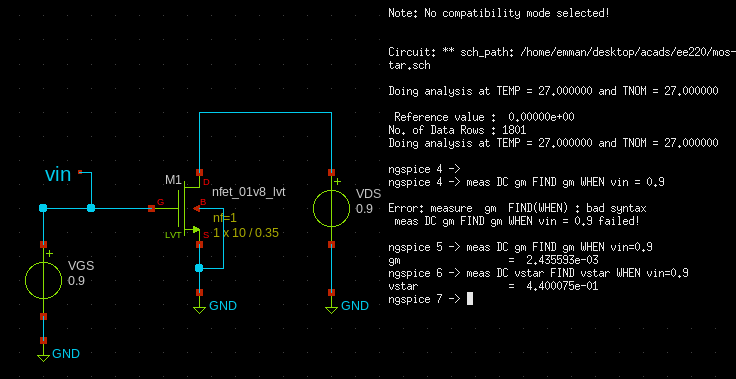
\includegraphics[scale=0.32]{gm-vstar.png}
	\label{fig:gm-vstar-NMOS} 
	\caption{$g_m$ and $v^*$}
\end{figure}
The values are obtained by using the MEAS command. Note that the TT corner is used.
\vspace{8pt}
\subsubsection{Simulations}
Flicker noise dominates the range $f < 500MHz$ whereas thermal noise dominates the region where $f > 500MHz$. With this, the flicker noise corner is at around $f=500MHz$. 
\begin{figure}[H]
	\centering
	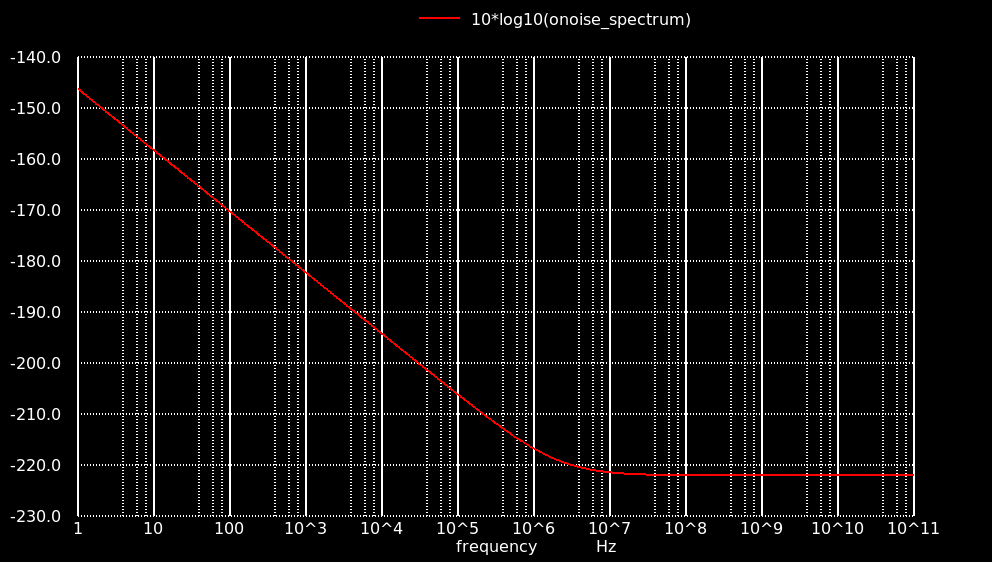
\includegraphics[scale=0.24]{noise-spectrum-35.png}
	\label{fig:noise-spectrum-35} 
	\caption{Output Noise PSD}
\end{figure}
\subsubsection{Estimating $\gamma$} Recall that in the absence of flicker noise, and assuming $\alpha=1$
\begin{equation*}
	\overline{i_{dn}^{2}} = 4kT\gamma g_{m} \Delta f
\end{equation*}
The total integrated noise power is equal to
\begin{align*}
	P_{i,noise} &= \int_{f1}^{f2}\overline{i_{dn}^{2}}\;df \\
	&= \int_{f1}^{f2} 4kT\gamma g_{m}\; df \\
	&= 4kT\gamma g_m \cdot (f_2 - f_1) 
\end{align*}
This means that if the integrated drain current noise power is obtained at the region where thermal noise is dominant, it is possible to directly compute for $\gamma$. To estimate the value of $\gamma$, the total output noise power with 10-GHz bandwidth from 90-GHz to 100-GHz is chosen. 
\begin{equation*}
	\gamma = \frac{P_{i,noise}}{4kTg_m(f_2-f_1)} 
\end{equation*}
In this case, 
\begin{equation*}
	\gamma \approx \frac{5.57E-13}{4kT\cdot 2.44E-3 \cdot 10E+9} = 1.375
\end{equation*}
We know that the total drain current noise is given by: 
\begin{align*}
		\overline{i_{dn}^{2}} &= \frac{K_f I_D}{C_{ox}L^2} \cdot \frac{\Delta f}{f} + 4kT\gamma g_{m} \Delta f \\    
		P_{i,noise} &= \int_{f1}^{f2}\overline{i_{dn}^{2}}\;df \\
		&= \frac{K_f I_D}{C_{ox}L^2} ln \left(\frac{f_2}{f_1} \right) + 4kT\gamma g_m \cdot (f_2 - f_1)
\end{align*}
In the simulation results, $P_{i,noise} = 6.336E-12$ 
By substituting the known values with $f_2 - f_1 = 100G$,  
\begin{equation*}
	\frac{K_f}{C_{ox}} = 8.439E-24
\end{equation*}
Upon increasing the length, the integrated drain current noise power is reduced. The flicker noise corner is at almost the same frequency. The reduction might be explained by the reduction in $g_m$ and $I_D$. Additionally, the flicker noise is inversely proportional to the square of the length. 

\newpage
\subsection{PMOS Noise}







\end{document}\textsl{}